%%%%%%%%%%%%%%%%%%%%%%%%%%%%%%%%%%%%%%%%%%%%%%%%%%%%%%%%%%%%%%%%%%%%%%%%%%%%%%%%

% Preamble

%%%%%%%%%%%%%%%%%%%%%%%%%%%%%%%%%%%%%%%%%%%%%%%%%%%%%%%%%%%%%%%%%%%%%%%%%%%%%%%%

% Page Settings
\documentclass[10pt]{report}
\usepackage[T1]{fontenc}
\usepackage[utf8]{inputenc}
\usepackage[letterpaper, margin=1in, left=1.5in]{geometry}

% Bibliography
\usepackage{biblatex}
\addbibresource{ref/thesis.bib}

% Packages and some formatting
\usepackage{titlesec,hyperref,booktabs,relsize,setspace,float,verbatim,caption,subcaption,graphicx}
%\hypersetup{colorlinks=true,linkcolor=blue,urlcolor=blue,citecolor=blue}
\hypersetup{hidelinks}
\titleformat{\chapter}[hang]
{\normalfont\huge\bfseries}{\chaptertitlename\ \thechapter:}{1em}{}
\doublespacing{}
\setcounter{tocdepth}{1}

% Identification
\title{}
\author{Christopher T. Tastad}
\date{day month year}

\begin{document}

%%%%%%%%%%%%%%%%%%%%%%%%%%%%%%%%%%%%%%%%%%%%%%%%%%%%%%%%%%%%%%%%%%%%%%%%%%%%%%%%

% Introductory Material

%%%%%%%%%%%%%%%%%%%%%%%%%%%%%%%%%%%%%%%%%%%%%%%%%%%%%%%%%%%%%%%%%%%%%%%%%%%%%%%%

% Title Page
\thispagestyle{empty}
\begin{center}
    \vspace*{1cm}

    \Huge
    \textbf{Refactoring the\\Candidate Cancer Gene Database}

    \vspace{1cm}
    \Large
    A Thesis\\
    SUBMITTED TO THE FACULTY OF THE\\
    UNIVERSITY OF MINNESOTA\\
    BY\\

    \vspace{1.5cm}

    \LARGE
    \textbf{Christopher T. Tastad}

    \vspace{3cm}

    \Large
    IN PARTIAL FULFILLMENT OF THE REQUIREMENTS\\
    FOR THE DEGREE OF\\
    MASTER OF SCIENCE\\

    \vspace{1cm}

    Adviser: Timothy K. Starr, PhD\\

    [full month and year of degree conferral]

\end{center}

% Copyright Page
\newpage
\thispagestyle{empty}

MIT License

Copyright (c) 2019 University of Minnesota

Permission is hereby granted, free of charge, to any person obtaining a copy of this software and associated documentation files (the ``Software''), to deal in the Software without restriction, including without limitation the rights to use, copy, modify, merge, publish, distribute, sublicense, and/or sell copies of the Software, and to permit persons to whom the Software is furnished to do so, subject to the following conditions:

The above copyright notice and this permission notice shall be included in all copies or substantial portions of the Software.

THE SOFTWARE IS PROVIDED ``AS IS'', WITHOUT WARRANTY OF ANY KIND, EXPRESS OR IMPLIED, INCLUDING BUT NOT LIMITED TO THE WARRANTIES OF MERCHANTABILITY, FITNESS FOR A PARTICULAR PURPOSE AND NONINFRINGEMENT\@. IN NO EVENT SHALL THE AUTHORS OR COPYRIGHT HOLDERS BE LIABLE FOR ANY CLAIM, DAMAGES OR OTHER LIABILITY, WHETHER IN AN ACTION OF CONTRACT, TORT OR OTHERWISE, ARISING FROM, OUT OF OR IN CONNECTION WITH THE SOFTWARE OR THE USE OR OTHER DEALINGS IN THE SOFTWARE\@.

%% Acknowledgements
%\newpage
\pagenumbering{roman}
%
%acknowledgements
%
%% Dedication
%\newpage
%
%dedication
%
%% Abstract
%\newpage
%
%abstract

\tableofcontents
\addcontentsline{toc}{chapter}{List of Tables}
\listoftables
\addcontentsline{toc}{chapter}{List of Figures}
\listoffigures

\newpage

\pagenumbering{arabic}

%%%%%%%%%%%%%%%%%%%%%%%%%%%%%%%%%%%%%%%%%%%%%%%%%%%%%%%%%%%%%%%%%%%%%%%%%%%%%%%%

% Introduction

%%%%%%%%%%%%%%%%%%%%%%%%%%%%%%%%%%%%%%%%%%%%%%%%%%%%%%%%%%%%%%%%%%%%%%%%%%%%%%%%


\chapter{Introduction}
Refactoring is intended to improve the design, structure, and/or implementation of the software (its non-functional attributes), while preserving its functionality. Potential advantages of refactoring may include improved code readability and reduced complexity; these can improve the source code's maintainability and create a simpler, cleaner, or more expressive internal architecture or object model to improve extensibility. Another potential goal for refactoring is improved performance; software engineers face an ongoing challenge to write programs that perform faster or use less memory\cite{Kerievsky2004}

\subsection{the challenge}

field of bio has ever increasing issues in data management and doesn't apply tech solutions very effectively. Ability to move past code to data manipulation and presentation. Deployment and the integration of common programming practices

In many ways, the field of Bioinformatics exists as the result of a problem rather than a discovery, as with other scientific fields. The nature of the challenges have evolved from a growth in the composition of primary data and a lacking compensatory set of technical skills to evaluate it. With the bottle neck that exists at the center of this problem, previously simple notions of collating, analyzing, and visualizing results no longer scale. As a result, a measurable area of focus is not just in the novel discovery of Biological relevance but in advancement of those engineer tools that offer new or dynamic means to solve old problems with new solutions.

\subsection{the tech has evolved}

Transitioning (implementing) existing solutions with new paradigms.  Improved data management (manipulation, collation, visualization).  Web front-end tech (web dev).  Technologies that enable reformed development (javascript, markdown, rstudio engine). Increased accessibility to non-tech users.

\subsection{applications of the tech in bio, specifically the CCGD}
gene screens in cancer bio~\cite{Clark2019}


Cancer gene screening is a hallmark case for this exploration as it lives at the nexus of being an area of high impact research and a process that can produce a deluge of raw data. In tandem, the state of web front ends has advanced in a manner that more completely allows~\cite{10.1093/nar/gkz1161}
In this work, we present a small but emblematic case that illustrates these shifting paradigms. With these incremental changeovers, no mater the impact, the field takes on a new character in the management of its growing data challenges. The CCGD as a concept set out to tackle some of these original problems of filtering handling large quantities of data. We expand on this by re-implementing the same achievement through a modern implementation.

%%%%%%%%%%%%%%%%%%%%%%%%%%%%%%%%%%%%%%%%%%%%%%%%%%%%%%%%%%%%%%%%%%%%%%%%%%%%%%%%

% Body

%%%%%%%%%%%%%%%%%%%%%%%%%%%%%%%%%%%%%%%%%%%%%%%%%%%%%%%%%%%%%%%%%%%%%%%%%%%%%%%%

\chapter{Body}

\section{Methods}

\subsection{Project Requirements}
This project's goal was ultimately to upgrade the existing CCGD\@. In setting out to do this, we established several requirements that took into consideration the opportunity to seize a routine set of server transitions to implement improved functionality. Specifically, the central output of the service should be retained in the eyes of the end user. Beyond this, attempting to fully reconstruct the backend provided for significant improvements (see Table~\ref{table:projectReqs}). These goals more broadly were: upgrade the existing server build to RHEL 7; rewrite web interface in a more modern framework; streamline the central table construction process using Rshiny; implement improved ability to manipulate table by product owner; employ improved software development best practices; generally seek opportunities for codebase and resource utilization improvements. Ultimately, all of these taken together were intended to serve some form of modernization and simplification.

\begin{table}[H]
    \caption{Project Requirements}\label{table:projectReqs}
    \relsize{-2}
    \addtolength\tabcolsep{-0.2em}
    \begin{tabular}{llllp{7cm}}
        \toprule
        &Feature&Goal&Framework&Description\\
        \midrule
        1&server OS&upgrade server OS&RHEL7&Transition of architecture for public server host. This is required by University OIT due to end of life schedule for RHEL6.\\
        \midrule
        2&web front-end&rewrite web interface&Rmarkdown&Improvements to the web interface written in a modern, simplified language. This will improved access to content creation and allow for automation in site rendering.\\
        \midrule
        3&table build&rewrite table build&Rshiny&Rshiny offers a dramatic improvement to replace the existing process by merging the table build back-end with a modern web display of the app interface.\\
        \midrule
        4&table update&improved admin controls&BASH/R&Existing app version confined some content controls to app author, preventing contributions by app owner.\\
        \midrule
        5&version control&implement best practices&git/docs&No version control was used in the original development of the app. This and other documentation practices were expanded in the rewrite\\
        \midrule
        6&n/a&resource improvements&codebase&Due to the lack of some best practices, there were many opportunities to make impactful resource improvements.\\
        \bottomrule
    \end{tabular}
    \addtolength\tabcolsep{+0.2em}
    \relsize{+2}
\end{table}

\subsection{Server Setup}
At it's core, the OS transition from RHEL 6 to 7 was the original project requirement that spurred this work. Existing hosting for the CCGD was owned by university OIT who established an end of life date for the current server OS\@. As a result, the bulk of core architecture implementation followed a narrow prescription for what was termed a ``Fully Managed'' RHEL7 install as detailed by the OIT-LPT Public-Docs~\cite{OIT}. Contrary to the implications of this installation name, a Fully Managed administration carried a mixture of privileges and management roles that were shared between OIT and our group. This was accomplished by leveraging a chef admin paradigm that was allowed limited sudo privileges within the hosted ecosystem. Importantly, items that extend from the core of server administration such as virtual machine creation, backups, and core security were handled by OIT\@. This left our group with the more focused task of administering exclusively our application.

[to what level of detail should i describe the server setup]

Apache

\subsection{Web Framework}
The upgraded build of the CCGD employed a completely different front-end architecture centralized around R web services environment. Built with dynamic modularity and data transportability in mind, the Rmarkdown framework offers the ability to render several independent markdown files into a unified website. We applied this feature set to produce our general site structure and content as it allowed for a massive simplification in web design. While following the existing site map, we recreated the raw content of the existing application as independent markdown files. Within the Rmarkdown format guide. The keystone feature of the Rmarkdown framework that allows for this unified rendering is the use of a YAML configuration header (see Figure~\ref{fig:siteYaml}). The \texttt{rmarkdown::render\_site} function leverages this configuration file to align and sequentially render content and styling in tandem for a complete site map [citeme rmarkdown docs]. Additionally, individual markdown pages employ this same configuration paradigm for page-specific parameters and formatting guidelines (see Figure~\ref{fig:pageHeader}).

\begin{figure}[H]
    
\includegraphics[width=\linewidth]{figs/rmarkdownflow.png}
    \caption{[TEMP] Rmarkdown Rendering Flow}\label{fig:renderFlow}
\end{figure}

[render diagram https://rmarkdown.rstudio.com/lesson-2.html]

responsive web design

An important distinction in summarizing the implementation of web framework is to point out that the Rshiny app, which contains the gene table, is assembled and hosted as a function separate from the general site rendering. More specifically to the web design, the shiny app is hosted at the common public repository \href{https://ctastad.shinyapps.io/table_app/}{\texttt{shinyapps.io}} and rendered in an inline iframe on the site search page. In the eyes of the user this presents a seamless transition, but the functional contrast permits for differential rendering between the two. This allows for the continuous integration of external sources that feed the table while eliminating the need to regularly render the static site content.

\begin{figure}
\centering
    \addtolength\tabcolsep{-0.2em}
    \relsize{-2}
\begin{subfigure}[b]{.5\linewidth}
    \centering
\begin{verbatim}
name: "Candidate Cancer Gene Database"
navbar:
    title: "CCGD"
    left:
        - text: "Home"
          href: index.html
        - text: "Search"
          href: search.html
        - text: "Help"
          href: help.html
        - text: "References"
          href: references.html
        - text: "Contact"
          href: contact.html
\end{verbatim}
\caption{\_site.yml: file for site assembly}\label{fig:siteYaml}
\end{subfigure}%
\begin{subfigure}[b]{.5\textwidth}
\centering
\begin{verbatim}
---
title: "Candidate Cancer Gene Database"
bibliography: refs/ccgd_paper.bib
nocite: '@*'
output:
    html_document:
        includes:
            in_header: "styles/favicon.html"
            after_body: "styles/footer.html"
        css: styles/styles.css
        theme: readable
---
\end{verbatim}
\subcaption{index.Rmd individual page header}\label{fig:pageHeader}
\end{subfigure}
\caption{YAML Configuration Segments}\label{fig:yamls}
    \addtolength\tabcolsep{+0.2em}
    \relsize{+2}
\end{figure}



\subsection{Rshiny App}
In order to replace the existing CCGD search functionality our group employed the Rshiny framework. Simply put, the shiny app that now enables this central purpose is an interactive web interface for a single table. Several changes were made to the existing integration pipeline in order to achieve this simplicity.

The structure of a general shiny app follows a highly reduced and consistent paradigm, and ours is no different. The broad format of this work flow is \texttt{ui + server $\rightarrow$ deployment}. The server specifically has a discrete composition made up of reactive constructs of inputs, expressions, and outputs that shape the app's reactive graph, which forms, more accurately, the discrete operation of the application. The assembly and movement of this graph is both emblematic and practical in displaying the modularity and improved resource utilization of the reactive elements. Without belaboring the description of reactive programming, this paradigm employs a declarative programming style that allows for lazy code execution~\cite{Wickham}. What this amounts to in application is for the developer to define loose controls at a higher level while allowing the code to passively fill these requirements. This translates to greater flexibility to both the developer and the machine as resource use can be reduced through modularity in code execution.

\begin{figure}[H]
    \centering
    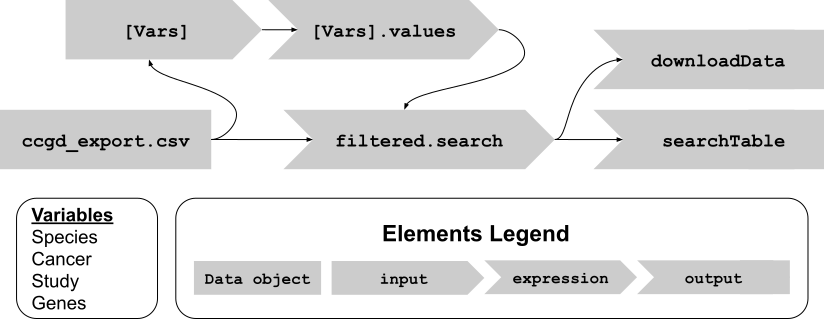
\includegraphics[width=\textwidth]{figs/g238.png}
    \caption{table\_app/app.R Reactive Graph}\label{fig:reactiveGraph}
\end{figure}

Within the scope of the \href{https://github.com/ctastad/ccgd/blob/master/table_app/app.R}{\texttt{table\_app/app.R}} server function we had a relatively simple goal of defining variable filters across the CCGD data table. Taking advantage of Rshiny's modularity, we created a two state path for the imported data object that allowed for both a variable-specific filter step along with a static, unchanged display of the table (see Figure~\ref{fig:reactiveGraph}). The advantage in doing this is that the table is displayed immediately on page load without the need to initiate a query. Additionally, the full, unfiltered table is available from the \texttt{downloadData} output at this state as well. For processing going down the filtered path, independent variable inputs are available to the user which are passed through two expression elements. In selecting a variable filter the \texttt{[Vars].values} expression applies a syntactic subsetting of the variable's data list which is then past to the central \texttt{filter.search} where the broader subsetting is carried to the rest of the table. The \texttt{searchTable} function takes the output of the filter and applies several text mutations to add external linking to several associated resources.

A small but fundamental element of our shiny app design was the use of the \texttt{renderDataTable} function in generating the \texttt{searchTable} output. The prior iteration of the CCGD architecture employed a relatively disproportionate MySQL database to store and serve numerous component elements that made up the table. Instead, the new implementation of our app now leverages the server-side processing capability of the DataTables JavaScript library. More specifically, we set parameters to create a reactive version of our function which allows for paging, searching, filtering, and sorting in real-time within the shiny server infrastructure [citeme DataTables]. Through this function alone we established new server paradigm that eliminated the MySQL database.

\subsection{Data Integration Process}

\subsection{Best Practices}
Some features of the software best practices from the previous version of the CCGD were done quite well such as the level of detail in the documentation. At the same time, many other important areas were missing in the development and maintenance of the application. Most prominent among these were the lack of any degree of version control and relatively inconsistent design principles. As a result, our group employed or improved upon several methods in an effort to elevate the quality, usability, and transportability of our codebase and application~\cite{Fincham2011}.

Throughout the course of the project we utilized a private github code repository for hosting and change tracking. This work has since been published on a public repository and assigned a DOI number through Zenodo~\cite{Tastad}. Furthering the spirit of project integrity, we expanded on the nature of the documentation for the user and, more prominently, the application owner. Specifically, documentation that was previously written in a Microsoft Word file was now recreated in markdown, and a notable tone and detail shift was made in serving the information transportability between administrators.

In approaching the process of development, we applied a philosophy of tidy code creation to both syntax and design. A supporting method in creating a more elegant code syntax was the use of R universe tools, tidyverse and Rmarkdown. Both offer a coding grammar that is centered around accessibility and simplification of high-level language organization~\cite{Wickham2019}. Furthering this simplification, we sought opportunities to deduplicate and extract subroutines in the table integration process in an effort to streamline resource constraints. Finally, another notable area for improvement we sought was in disk space utilization. The existing integration process relied on the continuous presence of what were several intermediary files that occupied a sizable disk capacity. To combat this we specifically reworked several data transformation steps to allow for the post-process elimination of these temporary data objects.

\section{Results}

\subsection{Architecture Upgrades}
previous installation used traditional lamp stack

Codebase reduction.

Need for sql database eliminated.

Interface improved. Table content contained within single page.

\begin{figure}[H]
    \centering
    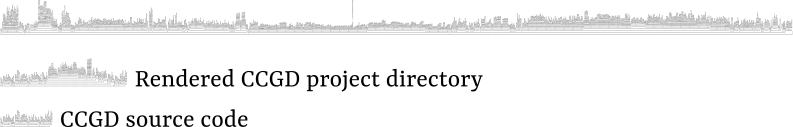
\includegraphics[width=\textwidth]{figs/g13732.png}
    \caption{Project directory file tree comparison}\label{fig:fileTree}
\end{figure}

Following the goals set out in our project requirements, we chose Rmarkdown as a replacement framework to develop the application's web front-end. Previously, the web interface for the application had been developed using Adobe Dreamweaver~\cite{Abbott2015}. For the time Dreamweaver served the purpose of simplifying the process of interface construction and web development, yet we hoped to extend the theme of simplified content creation into a modern framework. Further, utilizing a language such as Rmarkdown almost fully carries the development process into a state of pure content creation.

The original version of the CCGD front-end was developed using Dreamweaver~\cite{Abbott2015}. While this may have suitable at the time, several generations of web development have brought the field to be able to move beyond the process of design and focus more readily on content.

In an effort to reduce code complexity and improve access to content creation, an engineering choice was made to redesign the web front-end in Rmarkdown. While an approach such as this can reduce certain feature availability and overall design flexibility, a conscious priority was placed on the content of the page over the web functionality. In the spirit of our project goals,\ldots A framework such as Rmarkdown provides a development paradigm that dramatically shifts the effort of creation into that content rather than the creation broader page architecture [citeme rmarkdown docs]. The work of assembling that architecture is largely done for the user in leveraging

\subsection{Resource Utilization Improvements}
space constraints eliminated. Server resource reqs reduced overall.

\begin{figure}[H]
    \centering
    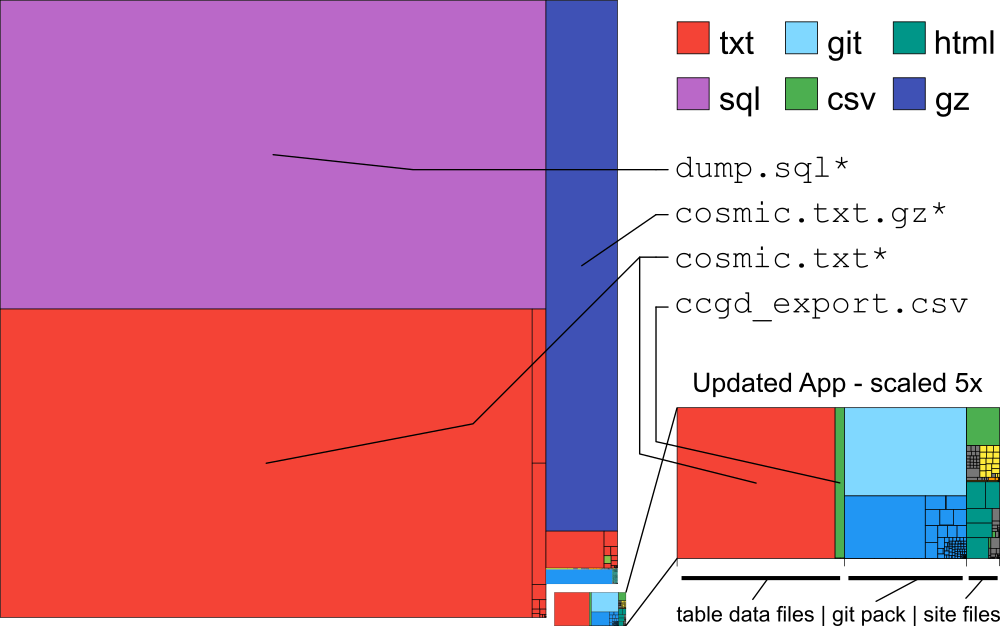
\includegraphics[width=\textwidth]{figs/g51565.png}
    \caption{Treemap of Disk Use Between App Versions}\label{fig:spaceTree}
\end{figure}

Ref crossdirstat

\subsection{Administration Streamlined}
server admin and app controls streamlined. Site render newly automated.

%%%%%%%%%%%%%%%%%%%%%%%%%%%%%%%%%%%%%%%%%%%%%%%%%%%%%%%%%%%%%%%%%%%%%%%%%%%%%%%%

% Conclusions

%%%%%%%%%%%%%%%%%%%%%%%%%%%%%%%%%%%%%%%%%%%%%%%%%%%%%%%%%%%%%%%%%%%%%%%%%%%%%%%%

\chapter{Conclusions}

Best practices. Discuss open source.

\addcontentsline{toc}{chapter}{Bibliography}
\printbibliography{}

\end{document}
